\section{Empirical Experiment}

In this section, we will first introduce a task with a low-dimensional continuous state-action space. This task can have different exploration difficulties by changing parameter configurations. Experiments on this task prove that our algorithm can achieve deep exploration. Then we modify the reward settings of the tasks on the Gym environment to be sparse or deceptive rewards. The results of these tasks show that our algorithm can solve more complex sparse reward tasks.

In the following experiments, we use the SAC algorithm with a double critical network and an automatic temperature adjustment as the baseline. By using the input of the last fully connected layer of one of the critics as the feature vector for calculating the Feature Matrix $\Lambda$, and selecting $ \beta = 10 $ as the coefficient of the UCB bonus. 

\begin{table*}[!htb]
    \centering
    \begin{tabular}{ccrrrrrrrrr}
    \toprule
    \multirow{2}{*}{$\Delta$} & \multirow{2}{*}{$1/\Delta$} &  & \multicolumn{2}{c}{well-defined task} &  & \multicolumn{2}{c}{sparse task} &  & \multicolumn{2}{c}{deceptive task} \\ \cline{4-5} \cline{7-8} \cline{10-11} 
                       &                      &  & $\beta=0.0$          & $\beta=10.0$         &  & $\beta=0.0$                 & $\beta=10.0$  &  & $\beta=0.0$           & $\beta=10.0$           \\ \hline
    0.0800             & 12.50                &  & 600            & 2200           &  & 1800                  & 3200    &  & 4100            & 3200             \\
    0.0700             & 14.29                &  & 700            & 2900           &  & 2800                  & 3600    &  & $>20000$           & 3600             \\
    0.0600             & 16.67                &  & 1200           & 3200           &  & 5100                  & 5000    &  & $>20000$           & 4500             \\
    0.0514             & 19.46                &  & 1300           & 3500           &  & 16600                 & 6100    &  & $>20000$           & 5200             \\
    0.0450             & 22.22                &  & 1700           & 3900           &  & $>20000$   & 8300    &  & $>20000$           & 7200             \\
    0.0400             & 25.00                &  & 2000           & 4600           &  & $>20000$   & 10800   &  & $>20000$           & 10600            \\
    0.0360             & 27.78                &  & 2400           & 5500           &  & $>20000$   & 11400   &  & $>20000$           & 13600            \\
    0.0327             & 30.56                &  & 2500           & 5100           &  & $>20000$   & 12700   &  & $>20000$           & 15200            \\ \bottomrule
    \end{tabular}
    \caption{Sample number need for solving different step coefficient $\Delta$ in well-defined, sparse and deceptive reward tasks }
    \label{tab:sample-number}
    \end{table*}

\subsection{Continuous Action Swim Task}
In order to measure the exploration ability of the proposed algorithm, we design a ``Swim'' task. This task has state space $ \mathcal{S} = [0,1]$, action space $ \mathcal{A} = [-1,1] $. Its state transfer function and reward function can be expressed by the following formula:

\begin{eqnarray}
    f(s) &=& -A \sin(2\pi \omega \cdot s) \\
    e(s,a) &=& \cos(\pi\cdot (a-f(s)))\\
    s'(s,a) &=& clip(s + \Delta \cdot e(s,a),0,1)\\
    r(s,a) &=& r_s\cdot s^l + r_a \cdot e(s,a)
\end{eqnarray}

\begin{figure}[!htb]
\centering
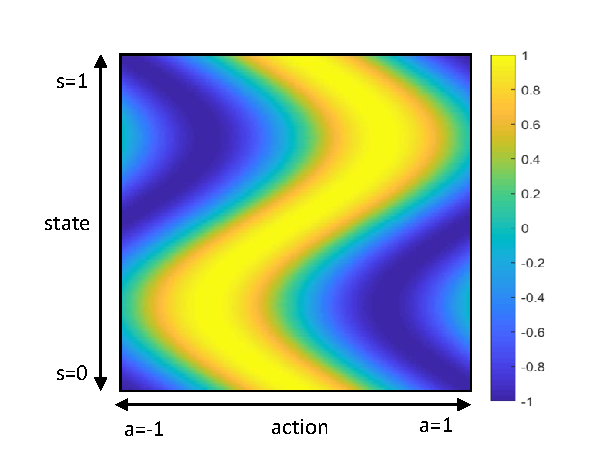
\includegraphics[width=230pt]{figs/Swim.pdf}
\caption{Effect $e(s,a)$ with $f(s) = -0.5\times \sin(2\pi\cdot s)$ in task Swim }
\label{fig:swim}
\end{figure}

Where $e(s,a)\in [-1,1] $ represents the effect of action $a$ in the state $s$, it reaches the maximum value $+1$ when $a=f(s)$ and reaches the minimum value $-1$ when $a= f(s)\pm 1 $. The effect affects both the state transition and the reward function. At each step, the state moves forward by $ \Delta \cdot e(s,a) $ and is truncated to the interval of $ [0,1] $. The task always starts at $ s_0 = 0 $ and resets after $ H = 100 $ steps. Each step of the reward includes two parts: the state reward $ r_s \cdot s ^ l $ and the action reward $ r_a \cdot e (s, a) $. The state reward is designed as a power function of $ s $ exponent $ l >> 1 $, so that the state reward is approximately distributed in the area of $ [1-1/l, 1] $. The action reward is designed to be proportional to the effect $ e(s, a) $ of the current action $ a $. When $ r_a> 0 $, it will guide the strategy forward, when $ r_a <0 $, it will guide the strategy back, and $ r_a = 0 $ has no guiding effect. These three cases correspond to "well defined", "deceptive", and "sparse", respectively.

\begin{figure}[!htb]
    \centering
       \subfigure[Sparse swim task with $\beta=10$]{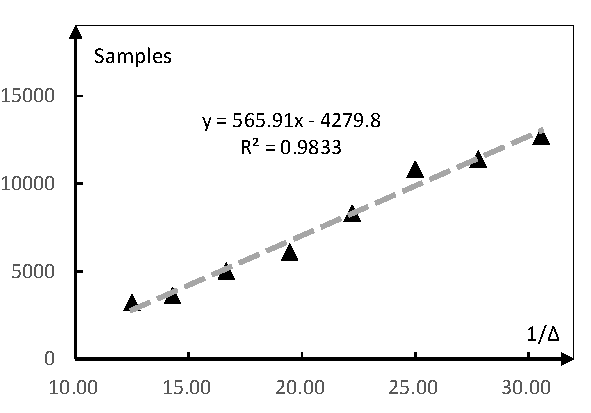
\includegraphics[width=180pt]{figs/Sparse.pdf}}
       \subfigure[Deceptive swim task with  $\beta=10$]{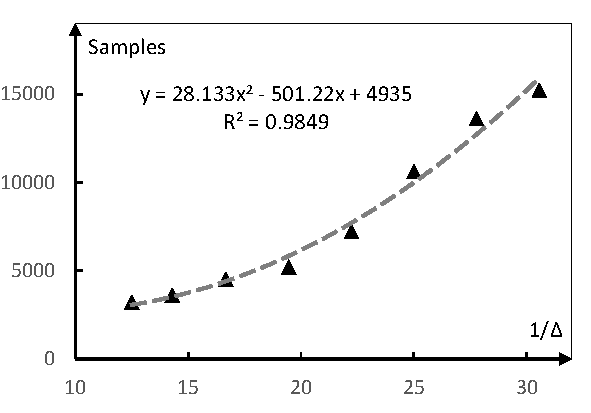
\includegraphics[width=180pt]{figs/Deceptive.pdf}}
    \caption{Scatter plot of $1/\Delta$-samples for sparse reward (top) and deceptive reward (down).}
   \label{fig:H-sample} 
\end{figure}
We perform experiments on different $ \Delta $ under the above three reward configurations. Each experiment is repeated ten times. We used the median curve to reach half of the reward when solving the task for the first time as the solving time of the task, and calculated the number of samples required to solve the task in each experiment as shown in the Table \ref{tab:sample-number}. The $>20000$ means the agent fail to reach state $s=1$ in $20000$ samples.

\begin{figure}[!htb]
    \centering
       \subfigure[Task with different $A$]{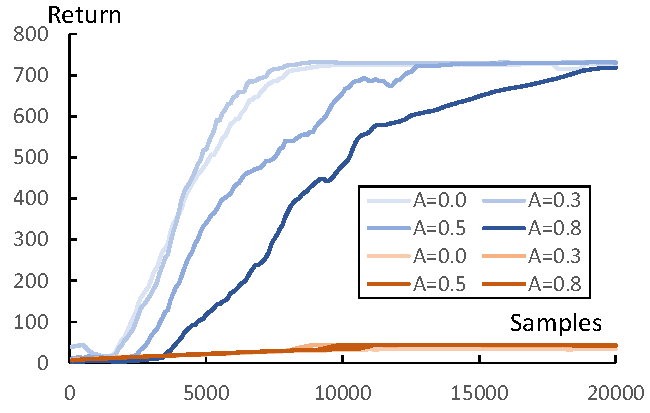
\includegraphics[width=180pt]{figs/A.pdf}}
       \subfigure[Task with different $\omega$]{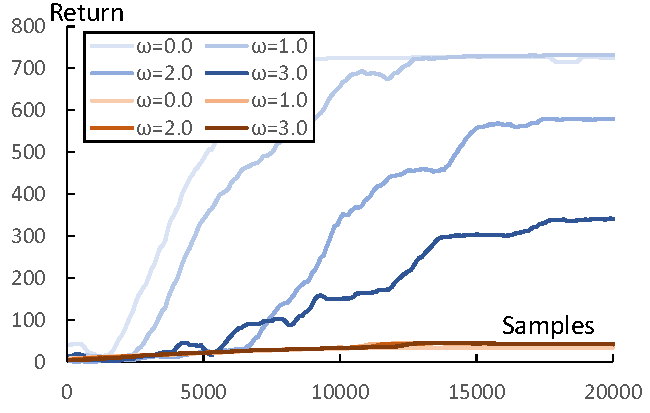
\includegraphics[width=180pt]{figs/f.pdf}}
    \caption{Mean return curve for different task configurations. The blue curve is $\beta = 10.0$ and the red is $\beta = 0.0$}
   \label{fig:A-f} 
\end{figure}

For a more intuitive understanding, we will plot the results on the sparse and deceptive tasks on the "$1/\Delta$-samples" axis in Fig \ref{fig:H-sample}. On sparse rewards, the sample required by our method to solve the task increases linearly with H, but has a square relationship on deceptive rewards. The algorithm that does not use the UCB bonus reward cannot quickly solve the task as $1/\Delta$ increases. This shows that our algorithm can effectively overcome bad reward shapes, and has the ability to improve the algorithm's deep exploration under different scales of $1/\Delta$.

In order to verify whether our algorithm can effectively solve the problem in more difficult situations, we also change other parameters of the task with deceptive rewards and evaluate the performance of the proposed method. Among them, $ A $ represents the best action changes with $ s $, and $ f $ represents the best action represents how often the best work changes with $ s $. The experimental results are shown in the Fig \ref{fig:A-f}.

Considering that the neural network fitting ability of finite neurons is limited, the convergence speed is slower for functions with large changes. The experimental results show that our algorithm can successfully solve the task under different task settings, and the baseline algorithm failed to solve any tasks even if the optimal action does not change with s ($ A = 0 $ or $ f = 0 $).

\subsection{Gym Experiment}

We have modified the reward settings for three continuous motion control tasks on Gym \cite{gym}: HalfCheetah and ContinuousMountainCar to make them sparse and deceptive rewards. 

\textbf{ContinuousMountainCar} \cite{MC}: In the ContinuousMountainCar, the agent needs to control a car from the bottom of the valley to the goal on the mountain top. The agent obtained reward $r = -\alpha*||\vec{a_t}||^2_2 + r_{goal}$ in each time step and the goal reward $r_{goal}=100$ only if the car reach the goal or zero otherwise. $\alpha=0$ in the sparse setting and $\alpha=0.1$ in the deceptive setting. The car needs to climb the left side first and then rush to the right side to reach the top of the mountain. Otherwise it can only oscillate back and forth in the valley.

\textbf{HalfCheetah}: In HalfCheetah, the agent need to control a half body cheetah in 2D space move forward. The agent receives $+1$ reward for each time step after the cheetah moves to the right beyond the distance $d$ and receives $-\alpha*||\vec{a_t}||^2_2$ action penalty.  $\alpha=0$ in the sparse setting and $\alpha=0.1$ in the deceptive setting.

We used both TD3 and SAC as our baseline algorithm and compared it with the method of constructing a LIFE bonus using the last layer of critical. The experiments for each setting repeat for 10 times and plot the mean return curve in Fig \ref{fig:GymCMC} and Fig \ref{fig:GymHC}.

\begin{figure}[hbt]
   \centering
   \subfigure[Sparse HalfCheetah task]{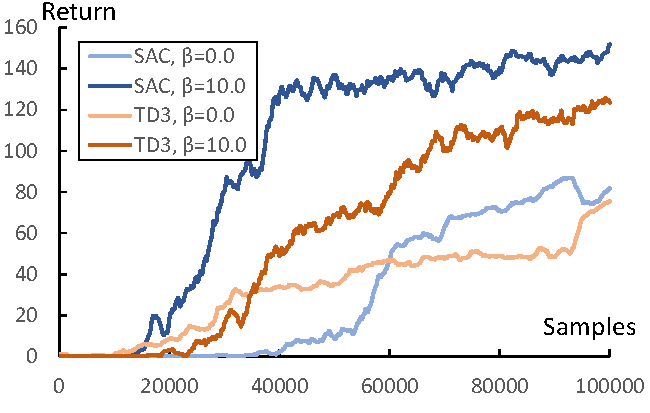
\includegraphics[width=180pt]{figs/SHC.pdf}}
   \subfigure[Deceptive HalfCheetah task]{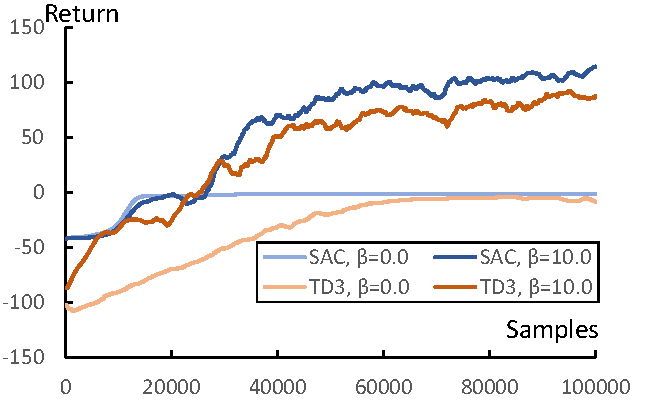
\includegraphics[width=180pt]{figs/DHC.pdf}}
   \caption{Mean return curve for SAC and TD3 on HalfCheetah task.}
   \label{fig:GymHC}
\end{figure}

\begin{figure}[hbt]
   \centering
   \subfigure[Sparse ContinuousMountainCar task]{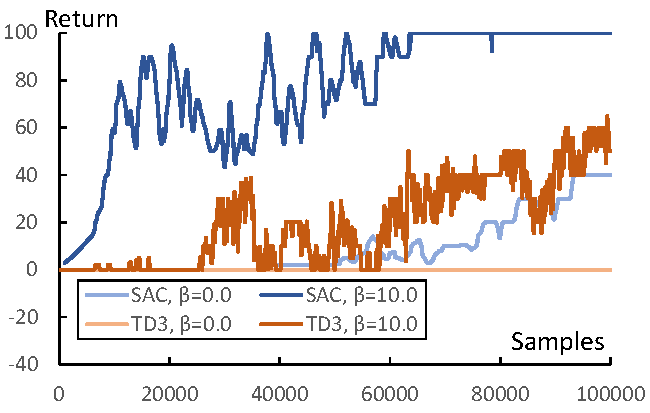
\includegraphics[width=180pt]{figs/SCMC.pdf}}
   \subfigure[Deceptive ContinuousMountainCar task]{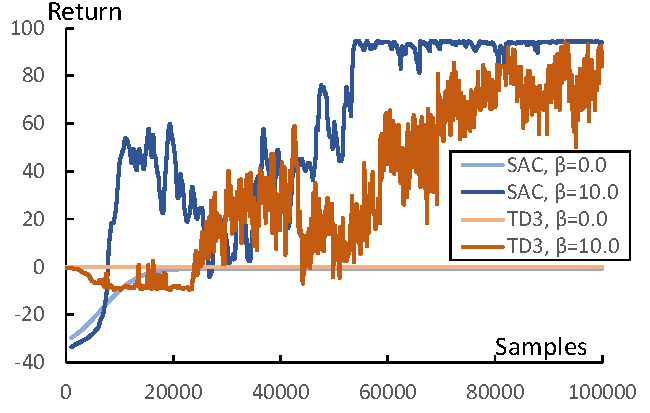
\includegraphics[width=180pt]{figs/DCMC.pdf}}
   \caption{Mean return curve for SAC and TD3 on ContinuousMountainCar task.}
  \label{fig:GymCMC} 
\end{figure}

It can be seen from the experimental results in Fig \ref{fig:GymCMC} and Fig \ref{fig:GymHC} that, in all tasks, the task using the LiFE bonus setting can be effective. In the case of $\beta = 10$, the agent can learn to reach the goal and continuously optimize the strategy. In the case of $\beta = 0$, the agent needs more samples to reach the goal or converges to the suboptimal strategy and stops in place.

In addition, we also found that the performance of the SAC algorithm on sparse and deceptive tasks is better than TD3. We consider that this is because the SAC algorithm uses a maximum entropy method that automatically adjusts parameters. The $\sigma$ of the Gaussian actor is relatively high at the beginning of training, resulting in a high exploration level and increasing the probability of visiting the goal. The average entropy of the actor will decrease with the training progress and converge to the optimal policy. TD3 relies on fixed action noise on the actor for exploration, and the exploration ability is limited. However, the maximum entropy strategy is a non-directional exploration method, so deep exploration cannot be achieved. The results indicate that combining deep exploration strategies such as LiFE bonus will achieve higher sample efficiency.